\section{Evaluation}\label{sec:eval}

We evaluate \( \tool \) based on the following four research questions:
\begin{itemize}
  \item RQ2) \textbf{Effectiveness} Is \( \tool \) effective to extract syntax and
    semantics of existing ECMAScript specifications?
  \item RQ1) \textbf{Correctness} Does \( \tool \) correctly extract JavaScript syntax
    and semantics from ECMAScript 2020 speicification?
  \item RQ3) \textbf{Adaptability} Does \( \tool \) deal with future proposed features?
  \item RQ4) \textbf{Specification Error Detection} What specification errors
    are detected by \( \tool \)?
\end{itemize}

\subsection{Effectiveness}

\begin{figure}[t]
  \centering
  \begin{subfigure}{0.23\textwidth}
    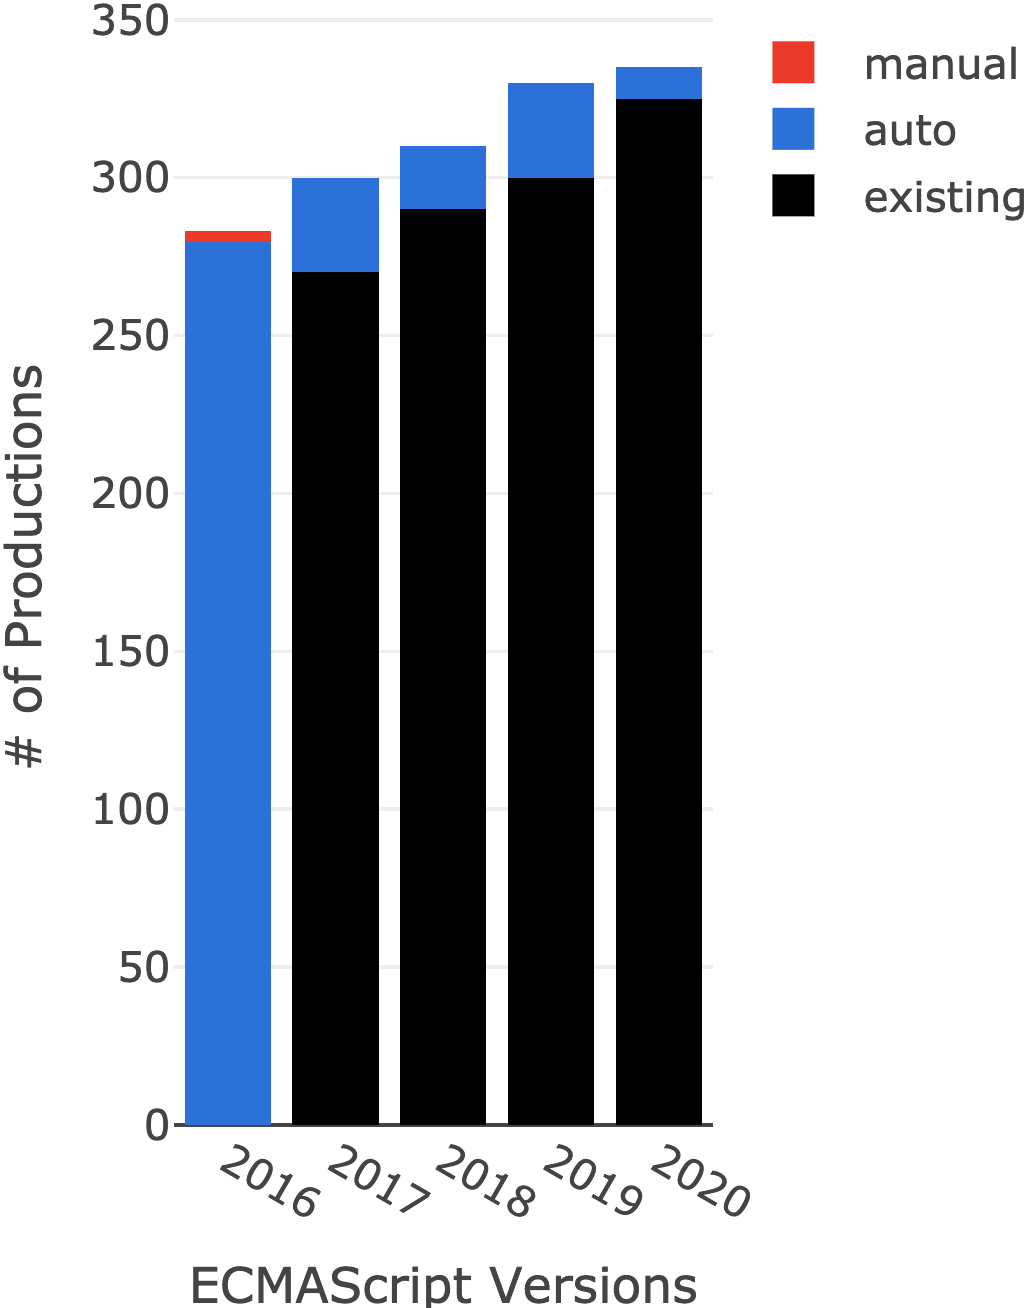
\includegraphics[width=\textwidth]{img/all-version-syntax.png}
    \caption{The parser generator.}
    \label{fig:syntax-all-version}
  \end{subfigure}
  \hfill
  \begin{subfigure}{0.23\textwidth}
    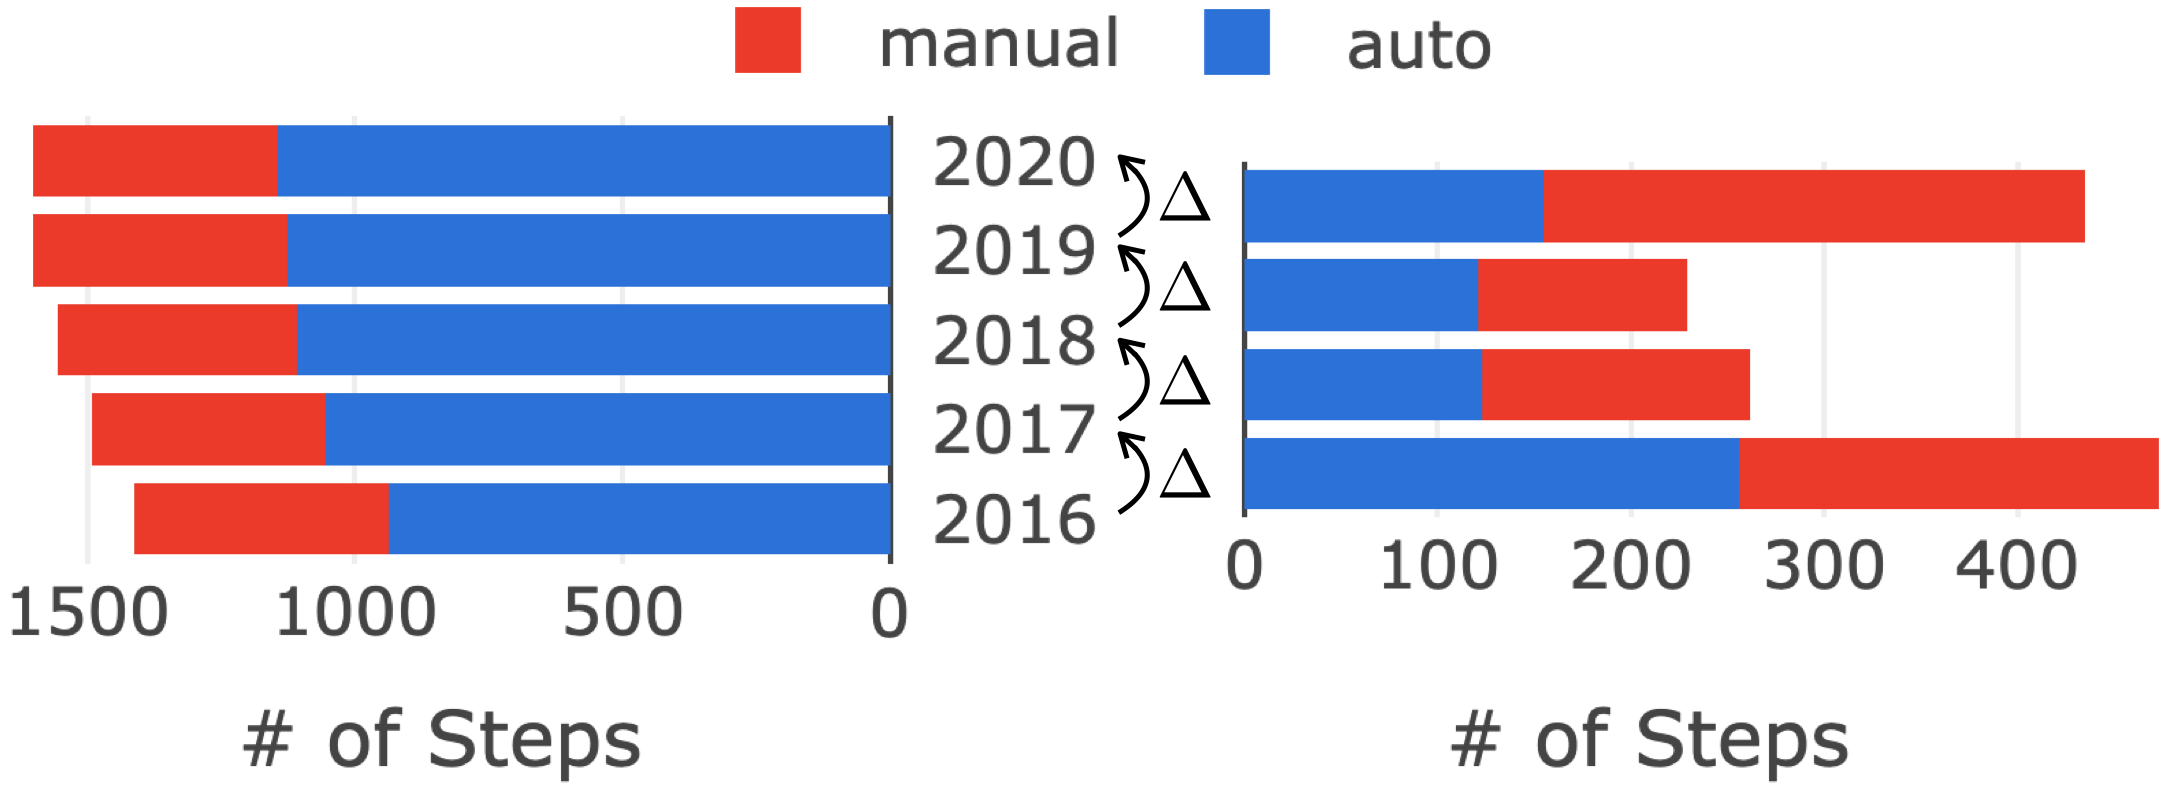
\includegraphics[width=\textwidth]{img/all-version-sem.png}
    \caption{The algorithm compiler.}
    \label{fig:semantics-all-version}
  \end{subfigure}
  \caption{The result of the parser generator and the algorithm compiler for
  ECMAScript specifications from 2016 to 2020.}
  \label{fig:all-version}
\end{figure}

We disucss the effectiveness of \( \tool \) by checking that the parser generator
and the algorithm compiler are able to handle existing ECMAScript specifications.
Figure~\ref{fig:all-version} shows the result of \( \tool \) from ECMAScript 2016
to 2020. While ECMAScript 5.1 is the first version that officially supports
the specification in HTML. However, two oldest versions ECMAScript 5.1 and 2015 are written
in quite different styles with recent versions including HTML tags used in abstract algorithms.
Thus, we evaluate only five recent versions from ECMAScript 2016 to 2020.
We first apply \( \tool \) into ECMAScript 2016 and counts how many productions in syntax
and algorithm steps in semantics are automatically extracted. For ECMAScript 2017 to 2020,
we consider only newly added productions and algorithm steps in ecah version.
For syntax, the parser generator successfully generates parsers for all \inred{XXX} productions
in ECMAScript 2016 and \inred{XXX} new productions in ECMAScript 2017 to 2020.
For semantics, the algorithm compilear successfully compiles \inred{XXXX} of \inred{XXXX} steps
into \( \ires \) instructions for ECMAScript 2016, and \inred{XXXX} of \inred{XXXX} newly added
steps are compiled in ECMAScript 2017 to 2020.

\subsection{Correctness}

\begin{table}[] \centering
  \begin{tabular}{lr}\toprule
    \belowrulesepcolor{gainsboro}
    \rowcolor{gainsboro} \textbf{All tests262 Tests} & \textbf{36,794} \\
    \aboverulesepcolor{gainsboro}\midrule
    Annexes/Internationalisation & 1,774\\ \hdashline
    In-process features & \inred{XXXX} \\\midrule
    Module tests & \inred{XXXX} \\\hdashline
    Non-strict tests & \inred{XXXX} \\\hdashline
    \belowrulesepcolor{gainsboro}
    \rowcolor{gainsboro} \textbf{ECMAScript 2020 Strict Script Tests} & \textbf{\inred{XXXXX}} \\
    \aboverulesepcolor{gainsboro}\midrule
    Not supported features & \inred{XXXX} \\\midrule
    \belowrulesepcolor{gainsboro}
    \rowcolor{gainsboro} \textbf{Applicable Tests} & \textbf{\inred{XXXXX}} \\
    \aboverulesepcolor{gainsboro}\midrule
    Passed tests & \inred{XXXX} \\\hdashline
    Failed tests & \inred{XXXX} \\\bottomrule
  \end{tabular}
  \caption{The syntax testing results of ECMAScript 2020 with test262.}
  \label{table:test262}
\end{table}

To check that \( \tool \) correctly extracts semantics, we apply our tool into ECMAScript 2020
specification. It is the next version of ECMAScript that is actively updated in GitHub~\ref{es2020}
to be released in the next year. Ecma Technical Committee 39 (TC39) officially provides
the conformance test suite, test262, for ECMAScript 2020. Thus, we develop \( \ires \)
interpreter to evaluate the \( \ires \) compiled from tests in test262.
However, test262 also provides tests for in-process features and other extensions
such as web browsers and internationalisation.
Thus, we exclude such tests from test262 test suite for evaluations.
Figure~\ref{table:test262} describes how to break down tests and the test results for parsers
and interpreters. We fixed the version of ECMAScript 2020 and test262 in August in 2019.
In that version, the test262 consists of 36,794 tests and we first exclude \inred{XXXX} tests
for extensions and in-process features. Then, we focus on only strict script not non-strict
or module codes thus we remove \inred{XXXX} tests. Finally, we have \inred{XXXX}


Then, we filter out tests having not supported features explained in Section~\ref{sec:framework}.
Table~\ref{table:}
We first exclude tests about not-yet applied proposed features, 

\subsection{Adaptability}
\subsection{Specification Error Detection}


% test262 결과를 어떻게? 전체 개수 / applicable tests 개수 / succes, fail 개수
% \inred{refactoring for compile rules / get statistics of compile rules}
% 개수만 - stmt / expr / cond / ref 몇개씩? / corner cases 개수
% \inred{proposed language features / related tests in test262 / diff of compile rules}
% 각 feature name / 의미 / compile 성공률 / 결과 test
% \inred{supprot "Assert: ... "?/ confirm found spec errors by TC39}
